\chapter{GPDs and Quark Distributions in Transverse Space}

\section{Introduction}

The challenge of understanding nucleon electromagnetic structure still 
continues after five decades of experimental scrutiny. From the initial 
measurements of elastic form factors to the accurate determination of 
parton distributions through deep inelastic scattering (DIS), the
experiments have increased in statistical and systematic accuracy.  Only 
recently it was realized that in fact the parton distribution functions
represent special cases of a more general, much more powerful, way to 
characterize the structure of the nucleon, the generalized parton 
distributions (GPDs)~\cite{Ji:1996nm,Ji:1996ek,Radyushkin:1996nd,
Radyushkin:1997ki}.  The GPDs are the Wigner quantum phase space 
distribution of quarks in the nucleon -- functions describing the 
simultaneous distribution of particles with respect to both position and 
momentum in a quantum-mechanical system, representing the closest analogue 
to a classical phase space density allowed by the uncertainty principle. 
In addition to the information about the spatial density (form factors) 
and momentum density (parton distribution), these functions reveal the 
correlation of the spatial and momentum distributions, {\it i.e.} how the 
spatial shape of the nucleon changes when probing quarks and gluons of 
different wavelengths.

The concept of GPDs has led to completely new methods of ``spatial imaging''
of the nucleon, either in the form of two-dimensional tomographic images 
(analogous to CT scans in medical imaging), or in the form of genuine 
three-dimensional images (Wigner distributions).  GPDs also allow us to 
quantify how the orbital motion of quarks in the nucleon contributes to the 
nucleon spin -- a question of crucial importance for our understanding of 
the ``mechanics'' underlying nucleon structure.  The spatial view of the 
nucleon enabled by the GPDs provides us with new ways to test dynamical 
models of nucleon structure. 

The mapping of the nucleon GPDs, and a detailed understanding of the
spatial quark and gluon structure of the nucleon, have been widely 
recognized as the key objectives of nuclear physics of the 
next decade. This requires a comprehensive program, combining results
of measurements of a variety of processes in electron--nucleon 
scattering with structural information obtained from theoretical studies, 
as well as with expected results from future lattice QCD simulations.

GPDs, in basic terms, describe the structure of the nucleon probed in 
reactions in which a high-energy, short-distance probe interacts with a 
{\em single quark} in the nucleon.  Mathematically, this is the 
quantum-mechanical amplitude for ``taking out'' a quark from the wave 
function of a fast-moving nucleon and ``putting it back'' with different 
momentum, thereby imparting a certain momentum transfer to the nucleon.
It depends on the fractions of the nucleon momentum carried by the
quark before and after the process, $x+\xi$ and $x-\xi$ ($\xi$ defines the 
longitudinal momentum transfer to the nucleon), as well as on the transverse 
momentum transfer to the nucleon, $\bm{\Delta}_\perp$.  In the special case 
of zero momentum transfer, $\xi = 0$ and $\bm{\Delta}_\perp = 0$, this 
amplitude reduces to the usual parton density of quarks in the nucleon, 
measured in inclusive deep-inelastic $eN$ scattering.  Similarly, in the 
case of non-zero transverse momentum transfer, $\bm{\Delta}_\perp \neq 0$, 
the integral of the GPD over $x$ reduces to the nucleon form factor at 
invariant momentum transfer $t = -\bm{\Delta}_\perp^2$, measured in elastic 
$eN$ scattering. Thus, the GPDs combine the traditional concepts of parton 
density and elastic form factor within a single structure.  The presence of 
spin -- both of the nucleon and the quark -- as well as quark flavors 
($u$, $d$, $s$) leads to the appearance of various independent spin/flavor 
components of the GPDs.  Together, they provide a comprehensive description 
of the quark structure of the nucleon.

The GPDs, however, contain much more information than the parton densities 
and elastic form factors alone. They describe the correlation of the quark 
longitudinal momenta ($x+\xi, x-\xi$) with the transverse momentum transfer 
to the nucleon ($\bm{\Delta}_\perp$).  This information permits a simple 
interpretation in terms of a spatial distribution of quarks in the nucleon. 
For $\xi=0$, the two-dimensional Fourier transform of the GPD with respect to 
$\bm{\Delta}_\perp$ describes the distribution of quarks with longitudinal 
momentum fraction $x$ over the transverse distance, $\bm{b}$, from the center 
of the nucleon (impact parameter).  The integral of this spatial distribution 
over $\bm{b}$ gives the total parton density at a longitudinal momentum 
fraction $x$.  This 1+2-dimensional ``mixed'' momentum and coordinate 
representation corresponds to a set of ``tomographic images'' of the quark 
distribution in the nucleon at fixed longitudinal momentum, $x$. 

A fully 3--dimensional spatial image of the nucleon is obtained when taking 
the Fourier transform of the GPD also with respect to the longitudinal 
momentum transfer to the nucleon, $\xi$, thus localizing the nucleon also in 
longitudinal space. In this case the GPD turns into the Wigner phase space 
distribution of quarks in the nucleon, describing their simultaneous 
distribution with respect to longitudinal momentum $x$ and the conjugate 
coordinate. A quantum phase space distribution describes the distribution
of particles over both coordinate and momentum (or, more generally,
pairs of conjugate variables) in a quantum mechanical system and
represents the closest analogue to a classical phase space density 
allowed by the uncertainty principle.  Fig.~\ref{fig:wigner} shows the 
spatial shape of the nucleon (contours of equal density) for quarks of 
different longitudinal momentum fraction, $x$, as obtained from a model GPD 
consistent with present parton density and form factor data. One sees 
that the effective shape of the nucleon changes with the quark 
momentum fraction probed in a certain reaction. This new 3D representation 
offers unprecedented possibilities not only for visualizing the nucleon as an 
extended object in space, but also for understanding the space-time evolution 
of scattering processes probing the quark and gluon structure of the nucleon.

%%%%%%%%%%%%%%%%%%%%%%%%%%%%%%%%%%%%%%%%%%%%%%%%%%%%%%%%%%%%%%%%%%%%%%%%
\begin{figure}[t]
\vspace{5.0cm}
\special{psfile=../der/wigner.eps hscale=70 vscale=70 hoffset=40 voffset=0}
\caption{\small{``3D images'' of the nucleon as obtained from a model phase 
space distribution incorporating phenomenological information about GPDs.
Shown are constant-density surfaces of the spatial distribution of $u$-quarks, 
for three values of the momentum fraction $x$.  In the valence quark region 
($x \geq 0.1$) the nucleon has a spherical shape. At large $x$ the size 
shrinks and the shape becomes oblate (disk-like). At small $x$, the quarks 
spread out in the longitudinal direction, and the shape becomes prolate 
(cigar-like).}}
\label{fig:wigner}
\end{figure}
%%%%%%%%%%%%%%%%%%%%%%%%%%%%%%%%%%%%%%%%%%%%%%%%%%%%%%%%%%%%%%%%%%%%%%%%

Further motivation for the study of GPDs comes from the fact that certain 
moments of the GPDs -- integrals over the quark momentum fractions -- are 
related to fundamental static properties of the nucleon that cannot directly 
be accessed experimentally otherwise.  In particular, the second moment of 
the GPDs gives the fraction of the nucleon spin carried by the quarks, 
including their spin and orbital angular momentum. Starting with the 
historic measurements by the EMC collaboration 20 years ago, determining 
how the spin of the nucleon is composed from the spins of the quarks and 
gluons and their orbital motion has been the central goal of polarized 
deep-inelastic scattering experiments.  Measurements of the GPDs would give 
access to the quark orbital angular momentum, thus providing information 
about another crucial piece of the nucleon ``spin puzzle''. 

The momentum transfer, $Q^2$, in $eN$ scattering defines the spatial 
resolution of the probe.  The description of hard exclusive processes in 
terms of GPDs applies to the limit of large $Q^2$, where the reaction is 
dominated by the scattering from a single, quasi-free quark (``leading--twist 
approximation'').  At lower $Q^2$, effects related to the interaction of 
quarks during the hard scattering process, or coherent scattering involving 
more than one quark, become important (``higher--twist effects'').  The 
minimum value of $Q^2$ required for the GPD description to be applicable in 
practice depends on the final state, and can ultimately only be determined 
experimentally.  For DVCS (see Fig.~\ref{fig:handbag}), the experience with 
inclusive DIS and other two-photon processes such as 
$\gamma^* \gamma \to \pi^0$ (measured in $e^+e^-$ annihilation) suggest that 
the leading-twist approximation should be reliable already at $Q^2 \sim$ few 
GeV$^2$.   Thus, DVCS can be used to extract information about GPDs at the 
momentum transfers accessible in fixed-target experiments.  For meson 
production, the experience with the pion form factor at high $Q^2$ and 
available meson electroproduction data suggest that higher-twist effects 
are significant up to momentum transfers of $Q^2 \sim$ 10-20~GeV$^2$. While 
such effects can be reduced by forming ratios of observables, or can be 
accounted for in phenomenological models, it seems likely that the use of 
meson production data for a quantitative extraction of GPDs requires 
measurements at significantly higher momentum transfers than in DVCS.

%%%%%%%%%%%%%%%%%%%%%%%%%%%%%%%%%%%%%%%%%%%%%%%%%%%%%%%%%%%%%%%%%%%%%%%%
\begin{figure}[t]
\vspace{5.0cm}
\special{psfile=../der/handbag.eps hscale=120 vscale=120 hoffset=-160 
voffset=-410}
\caption{\small{Reactions in $eN$ scattering probing the generalized parton 
distributions.  Deeply-virtual Compton scattering and meson production 
probe the GPDs at non-zero longitudinal and transverse momentum transfer, 
$\xi \neq 0, \bm{\Delta}_\perp = 0$. Different mesons ($\rho, \pi, K$) 
select different spin-flavor components of the GPDs.}}
\label{fig:handbag}
\end{figure}
%%%%%%%%%%%%%%%%%%%%%%%%%%%%%%%%%%%%%%%%%%%%%%%%%%%%%%%%%%%%%%%%%%%%%%%%

In the $eN \to eN\gamma$ cross section, the DVCS amplitude interferes 
with the known amplitude of the Bethe-Heitler (BH) process, in which the 
final-state photon is emitted from the electron (see Fig.~\ref{dvcsbh}). 
The total cross section is given by~\cite{Belitsky:2001ns}:

\begin{equation}
\frac{d\sigma^{e p \to e p \gamma}}{dx_B dy d\Delta^2 d\varphi} =
\frac{\alpha^3 x_B y}{16 \pi^2 Q^2 \sqrt{1+\epsilon^2}}
\left | \frac{\mathcal T}{e^3} \right |^2 \, ,
\end{equation}

\vskip 0.3cm

\noindent 
where $\epsilon=2 x_B M/Q$, $y$ is the fraction of the electron energy lost
in the nucleon rest frame and $\varphi$ is the angle between the leptonic
plane $(e,e')$ and the photonic plane ($\gamma^*,\gamma$).

%%%%%%%%%%%%%%%%%%%%%%%%%%%%%%%%%%%%%%%%%%%%%%%%%%%%%%%%%%%%%%%%%%%%%%%%
\begin{figure}[ht]
\centerline{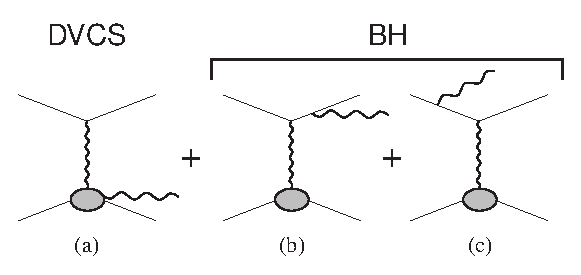
\epsfig{file=../der/diagbh.eps}}
\caption{\small{Diagrams contributing to the electroproduction of a real 
photon. The DVCS process (a) is shown along with the interfering Bethe-Heitler
diagrams (b) and (c).}} 
\label{dvcsbh}
\end{figure}
%%%%%%%%%%%%%%%%%%%%%%%%%%%%%%%%%%%%%%%%%%%%%%%%%%%%%%%%%%%%%%%%%%%%%%%%

The total amplitude $\mathcal T$ is the superposition of the BH and DVCS 
amplitudes:

\begin{eqnarray}
\left | \mathcal T \right |^2 & = & \left | \mathcal T_{BH} \right |^2+\left |
\mathcal T_{DVCS} \right |^2+ \mathcal I \\
\mathcal I & = & \mathcal T_{DVCS}^* \mathcal T_{BH} +
\mathcal T_{DVCS} \mathcal T_{BH}^* \, ,
\end{eqnarray}

\noindent 
where $\mathcal T_{DVCS}$ and $\mathcal T_{BH}$ are the amplitudes for the 
DVCS and Bethe-Heitler processes, and $\mathcal I$ denotes the interference 
between these amplitudes. The individual contributions to the total 
$e p \to e p \gamma$ cross section can be written as (up to twist-3 
contributions)~\cite{Belitsky:2001ns} as:

\begin{eqnarray}
\left| \mathcal T_{BH} \right|^2 & = & \frac{\Gamma_{BH}(x_B,Q^2,t)}{\mathcal P_1(\varphi) P_2(\varphi)}
\left\{ c_0^{BH} + \sum_{n=1}^2 c_n^{BH} \cos (n\varphi) +s_1^{BH} \sin\varphi \right\}  \, , \label{eq:epepgBH} \\
\left| \mathcal T_{DVCS} \right|^2 & = & \Gamma_{DVCS}(x_B,Q^2,t)
\left\{ c_0^{DVCS} + \sum_{n=1}^2 [ c_n^{DVCS} \cos (n\varphi) +s_n^{DVCS} \sin(n\varphi) ] \right\} \, , \label{eq:epepgDVCS} \\
\mathcal I & = & \frac{\Gamma_{I}(x_B,Q^2,t)}{\mathcal P_1(\varphi) P_2(\varphi)} ]
\left\{ c_0^{I} + \sum_{n=1}^3 [ c_n^{I} \cos (n\varphi) +s_n^{I} \sin(n\varphi) ] \right\} \, , \label{eq:epepgI}
\end{eqnarray}

\noindent 
where $\mathcal P_1(\varphi)$ and $\mathcal P_2(\varphi)$ are the BH electron 
propagators and $c_i,s_i$ are azimuthal moments in the corresponding cross 
section contributions.

Depending on whether the beam helicity or target spin is flipped, different 
GPD contributions enter the cross section azimuthal moments ($\sigma_{LU},
\sigma_{UL}$).  In practice, cross section asymmetries are experimentally 
easier to determine:

\begin{equation}
A=\frac{d\sigma^\leftarrow-d\sigma^\rightarrow}{d\sigma^\leftarrow+d\sigma^\rightarrow}\simeq\Gamma_A(x_B,Q^2,t)\frac{s_1^I \sin\varphi + s_2^I \sin 2\varphi}
{c_0^{BH}+c_0^I+\Gamma_Dc_0^{DVCS}+(c_1^{BH}+c_1^I+\Gamma_Dc_0^{DVCS})\cos\varphi} \, ,
\end{equation}

\vskip 0.3cm

\noindent 
where $\Gamma_A,\Gamma_D$ are  known kinematical prefactors. 

DVCS measurements thus allow one to separate the imaginary and real parts of 
the DVCS amplitude (\textit{cf.}\ Fig.~\ref{fig:handbag}) by measuring 
combinations of cross sections and asymmetries with respect to the beam spin 
(helicity), beam charge ($e^+/e^-$), and/or target or recoil polarization. 
The imaginary part of the amplitude probes the GPDs at $x=\xi = \xbj/2$,
the real part probes a certain integral over the quark momentum fractions. 

The different nucleon spin components of the GPDs can be extracted by 
measuring target spin asymmetries. Measurements of the $t$ ($\Delta_\perp$) 
dependence provide the information necessary for transverse nucleon imaging. 
Information about the flavor decomposition requires measurements with both 
protons and neutrons.   Additional information about the spin/flavor 
separation can come from meson production data. Studies of DVCS and meson 
production processes will require a combination of high energy and high beam 
intensity, and are generally much more challenging than traditional inclusive 
scattering experiments.

The {\tt CLAS12} setup will provide unprecedented capabilities for exploring 
nucleon structure in the valence quark region. In particular, it will provide
the  combination of high beam intensity (luminosity), high energy, high beam 
polarization, and advanced detection capabilities to provide a unique 
opportunity for studying nucleon GPDs in exclusive processes in the valence 
region.

\section{Present Experimental Results on Hard Exclusive Processes}

Measurements of exclusive processes at large momentum transfers 
have been carried out in $eN$ scattering experiments with existing 
fixed--target facilities (HERMES at DESY, JLab with 6~GeV beam 
energy) and the HERA collider. These studies have demonstrated the basic 
feasibility of such measurements, and have provided crucial evidence for 
the applicability of a GPD--based description of such processes.
They are also providing the first useful constraints for GPD phenomenology.

Experiments at fixed--target facilities aim to extract the
interference terms between the DVCS and the Bethe--Heitler (BH) amplitudes
in the $eN \to e'N\gamma$ cross section. The interference terms are 
experimentally accessible from combinations of measurements of the
spin--dependent and independent cross sections and relative asymmetries,
as well as from measurements of the beam charge dependence ($e^+ / e^-$)
of the cross section. In kinematic regions where the BH amplitude is much 
larger than the DVCS amplitude, the interference with the BH amplitude acts 
as a natural ``amplifier and filter'' for the DVCS amplitude, boosting
it to comfortably measurable levels. 

%%%%%%%%%%%%%%%%%%%%%%%%%%%%%%%%%%%%%%%%%%%%%%%%%%%%%%%%%%%%%%%%%%%%%%%%
\begin{figure}[ht]
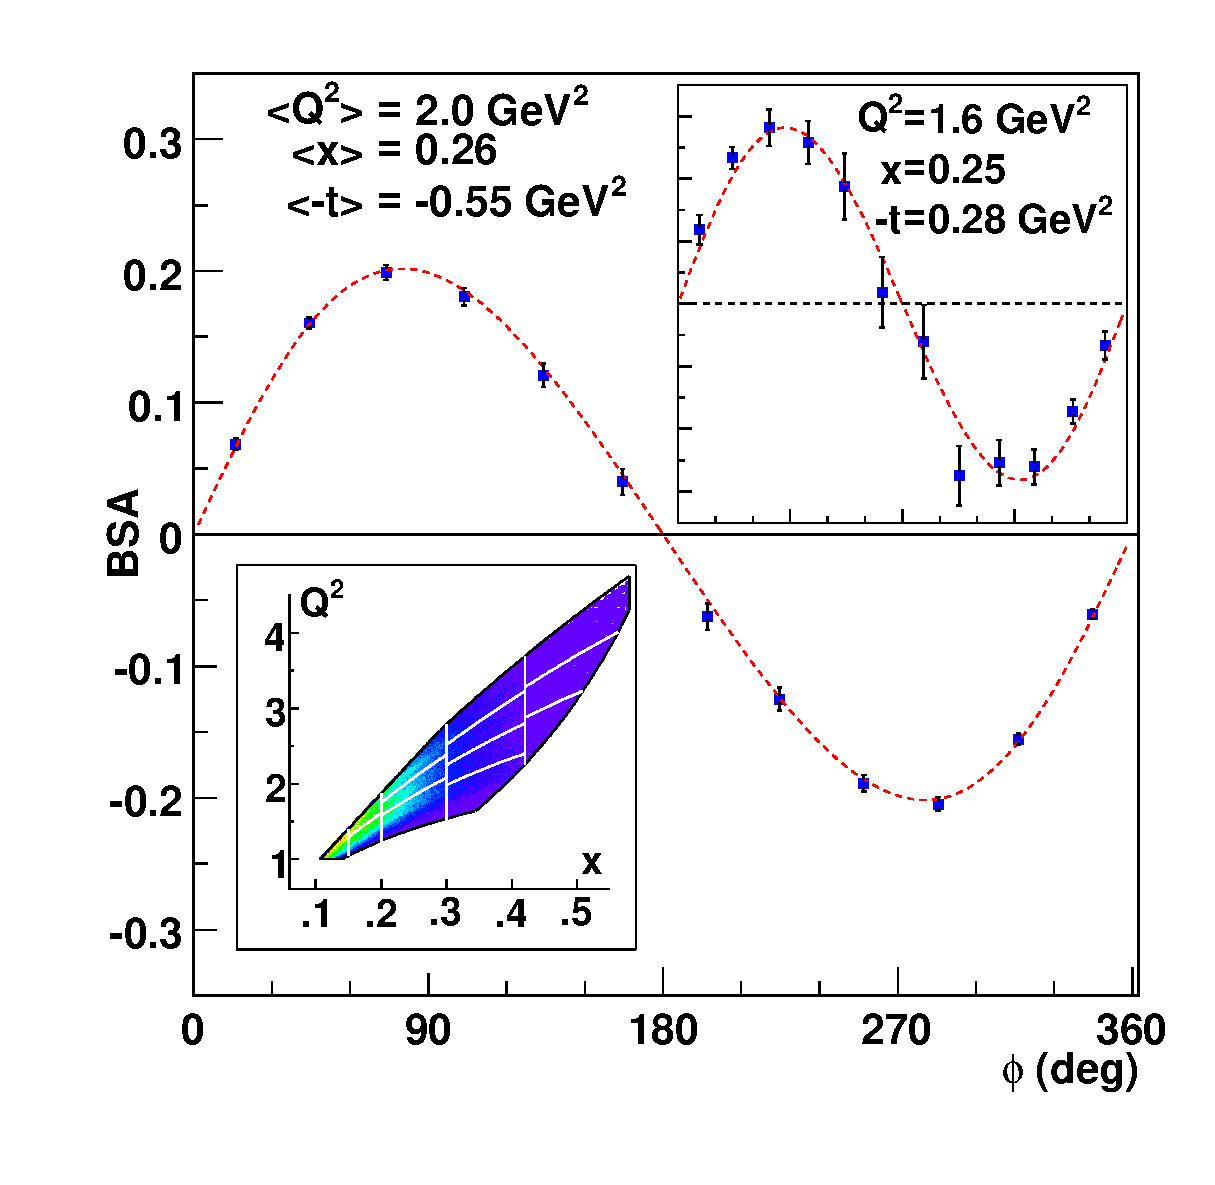
\includegraphics[width=0.99\textwidth]{../der/WP_CLAS_ALU.eps}
\caption{\small{Measurements of the beam spin asymmetry, $A_{LU}$, of the 
$eN \to e'N\gamma$ cross section from {\tt CLAS} at 6~GeV.  The plot in
the lower left corner shows the kinematic coverage in $\xbj$ and $Q^2$.
The main plot shows the beam spin asymmetry vs. $\phi$ integrated over all
kinematics (the average values are shown in the upper left of the plot.  In
the upper right of the plot, the beam spin asymmetry is shown for one of
our many kinematic points as an illustration.  The $\sin \phi$ dependence 
is characteristic of the BH-DVCS interference cross section.  The magnitude 
of the asymmetry can be related to a linear combination of the GPDs 
at $x = \xi$.}}
\label{fig:CLAS_e1}
\end{figure}
%%%%%%%%%%%%%%%%%%%%%%%%%%%%%%%%%%%%%%%%%%%%%%%%%%%%%%%%%%%%%%%%%%%%%%%%

Measurements of the beam spin asymmetry in $eN \to e'N\gamma$ have been 
performed by HERMES ($0.02 < \xbj < 0.3$)~\cite{Airapetian:2001yk}, {\tt CLAS}
\cite{Stepanyan:2001sm,JLabExp:E01-113} and Hall A ($0.15 < \xbj < 0.55$)
\cite{JLabExp:E00-110}.  Fig.~\ref{fig:CLAS_e1} shows the kinematic coverage 
of the {\tt CLAS} detector at 5.7~GeV, as well as the results for the 
asymmetry in a typical $(\xbj, Q^2)$ bin.  A new inner calorimeter was used 
to detect photons at small scattering angles.  The azimuthal angle dependence 
of the asymmetry clearly exhibits the $\sin\phi$ behavior characteristic
of the BH--DVCS interference. This asymmetry can be related to a linear 
combination of GPDs at $x = \xi$; the experimental results are consistent 
with the predictions of present GPD models. An important point is that with 
the {\tt CLAS} detector data in all $(\xbj, Q^2, t)$ bins are taken 
simultaneously, making it possible to extract information about the GPDs 
over a wide kinematic range.

While the unpolarized GPD $\cal H$ dominates the beam spin asymmetry at 
small $t$~\cite{Belitsky:2001ns}, $\sigma_{LU} \sim F_1{\cal H}-\xi F_2{\cal 
\widetilde H}$, the target single spin asymmetry at small $t$ has a 
significant contribution from the polarized GPD $\cal \widetilde H$
\cite{Belitsky:2001ns}: $\sigma_{UL} \sim F_1{\cal \widetilde H}-\xi 
F_2{\cal H}$.  Therefore, a combined analysis of the beam and target single 
spin asymmetries will allow for separation of $\cal H$ and $\cal \widetilde H$.

Recently published results by the {\tt CLAS} collaboration on the first 
measurements of the target spin asymmetry~\cite{Chen:2006na} confirmed again 
that the factorization is likely to be applicable at $Q^2$ values as low as 
2~GeV$^2$. These measurements eventually will allow one to separate the 
contributions from unpolarized and polarized nucleon GPDs.  An order of 
magnitude more data are expected from JLab during the next two years, which 
would allow for more accurate extraction of GPD parameters. 

The measurements of the DVCS cross sections and beam spin asymmetries carried 
out by JLab with 6~GeV beam energy support the theoretical expectation of 
dominance of the single-quark reaction mechanism (leading-twist approximation) 
for DVCS for momentum transfers $Q^2$ of a few GeV$^2$, essential for the GPD 
interpretation of the $eN \to e'N\gamma$ data.  They also demonstrate the 
feasibility of accurate differential measurements of the $t$-dependence of the 
cross sections needed for the GPD-based reconstruction of the spatial images 
of the nucleon.

The HERMES collaboration measured for the first time the beam charge 
asymmetry of the cross section, which probes a dispersive integral of the 
GPDs over the quark momentum fractions \cite{Airapetian:2006zr}.  DVCS 
cross sections at high $Q^2$ were measured at HERA
\cite{Chekanov:2003ya,Adloff:2001cn}, including its $t$-dependence; the 
results are well described by leading-order (LO) and next-to-leading order 
(NLO) QCD calculations incorporating QCD evolution of the GPDs, thus fully 
confirming the applicability of QCD factorization to exclusive processes 
at high energies.

\subsection{GPD Measurements with Jefferson Laboratory at 12 GeV}

{\tt CLAS12} will provide a unique combination of high beam intensity 
(luminosity), high energy, and large--acceptance detectors, which will 
enable studies of exclusive processes such as DVCS and meson production 
in the valence quark region.

%%%%%%%%%%%%%%%%%%%%%%%%%%%%%%%%%%%%%%%%%%%%%%%%%%%%%%%%%%%%%%%%%%%%%%%%
\begin{figure}[ht]
\centerline{\epsfig{file=../der/asymmetry_detail.eps,width=\linewidth}}
\caption{\small{On all figures: points in red represent data with statistical 
error bars. Lines are models with different input parameters, none of which 
includes twist-3 contributions:  The full line is a model with a Regge-type 
$t$-dependence and D-term. The dotted line includes the Regge-type 
$t$-dependence but has no D-term. The dash-dotted line has the D-term but the 
$t$ dependence only comes from form factors. Left figure: Beam spin asymmetry 
(BSA) as a function of $\varphi$ for $<x_B>=0.2$, $<Q^2>=3.3$~GeV$^2$, and 
$<-t>=0.45$~GeV$^2$. Middle figure: BSA as a function of $-t$ for $<x_B>=0.2$, 
$<Q^2>=3.3$~GeV$^2$, and $\varphi=90^\circ$. Right figure: BSA as a function 
of $x_B$ for $t=0.45$~GeV$^2$, $<Q^2>=3.3$~GeV$^2$ and $\varphi=90^\circ$.}}
\label{fig:asymbig}
\end{figure}
%%%%%%%%%%%%%%%%%%%%%%%%%%%%%%%%%%%%%%%%%%%%%%%%%%%%%%%%%%%%%%%%%%%%%%%%

Detection of the photon in the {\tt CLAS} inner calorimeter, in addition 
to the recoil proton and scattered electron, provides the exclusivity 
condition crucial for complete control over different background processes. 
Using the $epX$ sample  has its own advantages with regard to background 
suppression ($\pi^0$) and azimuthal angle coverage.  The two samples probe 
$ep \to e'\gamma p$ in regions of different relative magnitudes of the DVCS 
and Bethe-Heitler amplitudes.  In this way, GPDs can be extracted using both 
absolute cross section and polarization asymmetry data. The possibility to 
use both methods in experiments at a single facility represents a crucial 
advantage of {\tt CLAS12}.

%%%%%%%%%%%%%%%%%%%%%%%%%%%%%%%%%%%%%%%%%%%%%%%%%%%%%%%%%%%%%%%%%%%%%%%%
\begin{figure}[ht]
\begin{center}
\epsfig{file=../der/tsa_phi_comp.epsi, totalheight=15cm, width=6.5cm, angle=270}
\caption{\small{(a). Target spin asymmetry versus $\varphi$ for 
$Q^2$=4.1~GeV$^2$, $x_B$=0.36, and $-t$=0.52~GeV$^2$. The black points show 
the values from Ref.~\cite{Vanderhaeghen:1999xj} using CTEQ6 PDFs with the 
estimated errors from the proposed measurement. The red solid curve is using 
MRST02 PDFs with $E=\widetilde{E}$=0, and for the blue dashed curve is 
$\widetilde{H}$ is also set to zero. (b). $\sin{\varphi}$ moments of the 
target spin asymmetry versus $-t$ at $Q^2$=4.1~GeV$^2$ and $x_B$=0.36, and 
(c). versus $x_B$ at $Q^2$=4.1~GeV$^2$ and $-t$=0.52~GeV$^2$. The projected 
error bars represent the statistical uncertainties only.}} 
\label{Fig:TsaPhiComp}
\end{center}
\end{figure}
%%%%%%%%%%%%%%%%%%%%%%%%%%%%%%%%%%%%%%%%%%%%%%%%%%%%%%%%%%%%%%%%%%%%%%%%

To separate the different spin components of the GPDs, measurements of a 
variety of polarization observables (beam and target spin) will be performed. 
The longitudinal beam single spin asymmetry, $A_{LU}$ (see 
Fig.~\ref{fig:asymbig}), will access mainly the unpolarized Dirac GPD, 
$\cal H$.  Combined analysis of the DVCS data on a longitudinally polarized 
target single spin asymmetry (see Fig.~\ref{Fig:TsaPhiComp}) with the beam 
single spin asymmetry will provide separation of contributions from 
unpolarized and polarized GPDs.  The double spin asymmetry for longitudinal 
target polarization, $A_{LL}$, provides information on the real part of the 
corresponding GPDs, complementary to beam charge asymmetries.
 
The results of these measurements can directly be translated into transverse 
spatial images of the nucleon. As an example, Fig.~\ref{fig:H_proj} shows 
the projected results for the Dirac GPD, $\cal H$, as a function of $x$ and 
$t$, and its corresponding transverse spatial representation.  Complementary 
information can be obtained about integrals of the GPDs over the quark 
momentum fraction. With the help of GPD parameterizations, this information 
can be used to construct 2-dimensional tomographic images of the nucleon.

%%%%%%%%%%%%%%%%%%%%%%%%%%%%%%%%%%%%%%%%%%%%%%%%%%%%%%%%%%%%%%%%%%%%%%%%
\begin{figure}
\begin{tabular}{cc}
\parbox[c]{0.4\textwidth}{
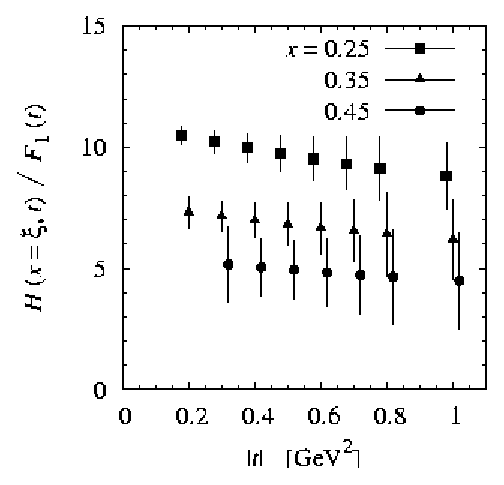
\includegraphics[width=0.4\textwidth]{../der/gpdtdep.eps}}
&
\parbox[c]{0.56\textwidth}{
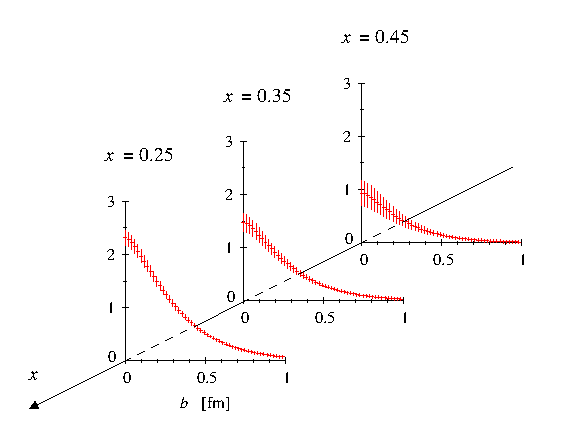
\includegraphics[width=0.56\textwidth]{../der/spatial_narrow.eps}}
\end{tabular}
\caption{\small{Left: Projected results for the Dirac GPD of the proton, 
${\cal H}(x = \xi, t)$, as a function of $x$ and $t$, as extracted from the 
DVCS beam spin asymmetry, $A_{LU}$, measured at JLab at 12~GeV. Shown is the 
ratio of the GPD to the the proton's Dirac form, $F_1(t)$.  Right: Transverse 
spatial image of the proton obtained by Fourier-transforming the measured GPD. 
The errors were estimated assuming a dipole-like $t$-dependence.}}
\label{fig:H_proj}
\end{figure}
%%%%%%%%%%%%%%%%%%%%%%%%%%%%%%%%%%%%%%%%%%%%%%%%%%%%%%%%%%%%%%%%%%%%%%%%

Additional information about the flavor structure of GPDs will come from 
ratios of meson production cross sections in channels with the same 
spin/parity quantum numbers, such as $\eta / \pi^0$ and $K^* / \rho^+$. 
These channels will be measured simultaneously with DVCS, not requiring any 
extra beam time.

Measurements of exclusive meson production in non-diffractive channels in
{\tt CLAS12} would allow for detailed studies of the spin, flavor, and 
spatial distributions of quarks in the nucleon in the valence region, 
complementing the information from DVCS measurements.  Very interesting 
information can already be gained by comparing observables for different 
mesonic channels, without detailed modeling of the GPDs.  For example, a 
comparison of $\pi^0$ and $\eta$ provides model-independent information 
about the ratio of the quark spin distributions $\Delta u$ and $\Delta d$ 
and their spatial distributions.  Comparison between $\pi^+$ and $K^+$ 
production, as well as between $\rho^+$ and $K^{*+}$, allows one to study 
$SU(3)$ flavor symmetry breaking in the nucleon's quark distributions in 
different spin/parity channels.  More information about the spatial 
distribution of quarks can be obtained from the GPD analysis of absolute 
cross sections ($\sigma_L$) in these channels.  Separation of the various 
response functions ($L$, $T$, etc.) would provide a crucial test of the 
dominance of the single-quark reaction mechanism at large $Q^2$.

Another interesting class of processes that could be studied are exclusive 
reactions with $N \to N^*$ transitions.  Such processes probe the 
``transition GPDs'' -- the probability amplitude for the nucleon to  
undergo a transition to an excited state when ``taking out'' a quark and 
``putting it back'' with different momentum. In these reactions the hard 
scattering process can be regarded as an operator inducing an $N \to N^*$ 
transition. {\tt CLAS12} is capable of performing such measurements requiring 
detection of decay products of the recoiling nucleon resonances.
